\documentclass[12pt, twoside]{article}
\usepackage[letterpaper, margin=1in, headsep=0.5in]{geometry}
\usepackage[english]{babel}
\usepackage[utf8]{inputenc}
\usepackage{amsmath}
\usepackage{amsfonts}
\usepackage{amssymb}
\usepackage{tikz}
\usepackage{yhmath}
%\usetikzlibrary{quotes, angles}

\usepackage{graphicx}
\usepackage{enumitem}
\usepackage{multicol}

\usepackage{fancyhdr}
\pagestyle{fancy}
\fancyhf{}
\renewcommand{\headrulewidth}{0pt} % disable the underline of the header

\fancyhead[RE]{\thepage}
\fancyhead[RO]{\thepage \\ Name: \hspace{3cm}}
\fancyhead[L]{BECA / Dr. Huson / 10th Grade Geometry\\* 14 June 2019}

\begin{document}
\subsubsection*{13.10 Do Now: Mixed review}
 \begin{enumerate}

  \item Given $m\angle R=30$ and $m\angle U=70$. Find $m\angle UST$.\\[1cm]
  \begin{tikzpicture}
   %\draw [->, thick] (0,0)--(5,5);
   \draw [<-, thick] (8,0)--(0,0)--(3,3)--(4.5,0);
   \draw [fill] (0,0) circle [radius=0.05] node[below]{$R$};
   \draw [fill] (4.5,0) circle [radius=0.05] node[below]{$S$};
   \draw [fill] (3,3) circle [radius=0.05] node[right]{$U$};
   \draw [fill] (7,0) circle [radius=0.05] node[below]{$T$};
  \end{tikzpicture} \vspace{1cm}

  \item Write down the center and radius of each circle.
   \begin{enumerate}
     \begin{multicols}{2}
     \item   $(x+1)^2+(y+3)^2=1$ \vspace{2.5cm}
     \item   $x^2+(y-4)^2=25$ \vspace{2.5cm}
     \end{multicols}
   \end{enumerate} \vspace{2cm}

  \newpage
  \item In the diagram below, $\overline{AC}$ has endpoints with coordinates $A(-3,1)$ and $C(6,4)$.
   \begin{center} %4 quadrant regents grid
     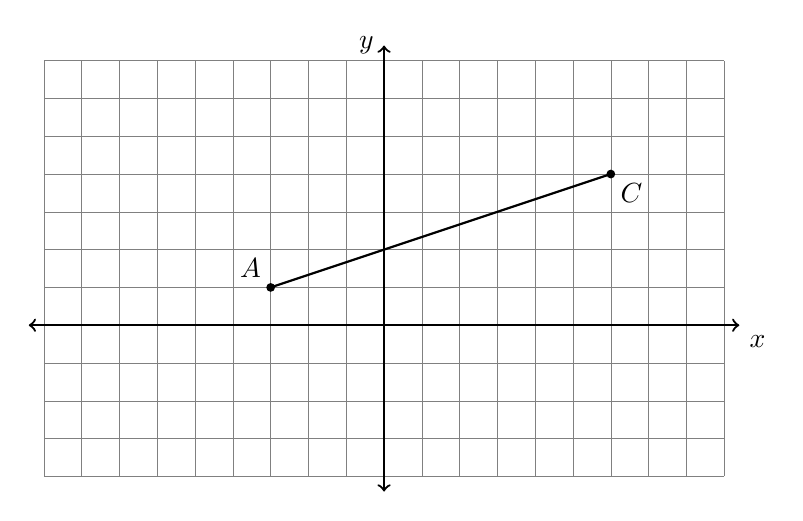
\begin{tikzpicture}[scale=.48]
       \draw [help lines] (-9,-4) grid (9,7);
       \draw [thick, <->] (-9.4,0) -- (9.4,0) node [below right] {$x$};
       \draw [thick, <->] (0,-4.4)--(0,7.4) node [left] {$y$};
       \draw [thick] (-3, 1)--(6,4);
       \draw [fill] (-3, 1) circle [radius=0.1] node[above left] {$A$};
       \draw [fill] (6, 4) circle [radius=0.1] node[below right] {$C$};
     \end{tikzpicture}
   \end{center}
   If $B$ is a point on $\overline{AC}$ and $AB {:} BC = 2{:}1$,  what  are  the coordinates of $B$? \vspace{4cm}

  \item Triangle $ABC$ is dilated with a scale factor of $k$ centered at $A$, yielding $\triangle ADE$, as shown. Given $AB=8$, $BC=10$, $AC=12$, and $DE=15$. \\[0.25cm] Find $BD$, $AE$, and $k$ (the scale factor).\\[0.25cm]
     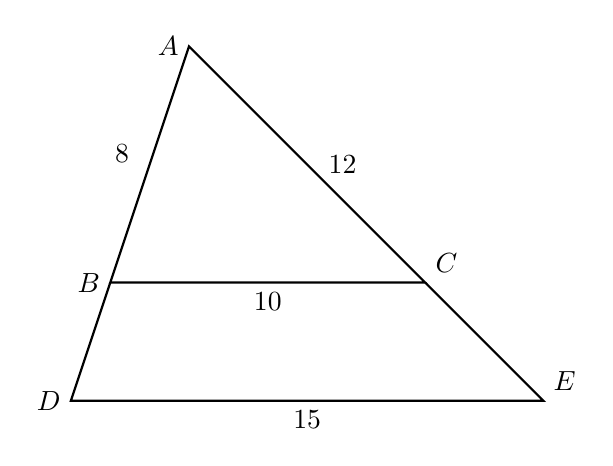
\begin{tikzpicture}[scale=0.5]
       \draw [thick]
       (0,0)node[left]{$B$}--
       (8,0)node[above right]{$C$}--
       (2,6)node[left]{$A$}--cycle;
       \draw [thick]
       (0,0)--
       (-1,-3)node[left]{$D$}--
       (11,-3)node[above right]{$E$}--(8,0);
       \node at (4,0)[below]{$10$};
       \node at (5.3, 3)[right]{$12$};
       \node at (0.3, 2.8)[above]{$8$};
       \node at (5,-3)[below]{$15$};
     \end{tikzpicture}
  \vspace{2cm}

  \item What transformation maps $\triangle ABC$ onto $\triangle DEF$, shown below? Fully specify the transformation.
    \begin{center}
      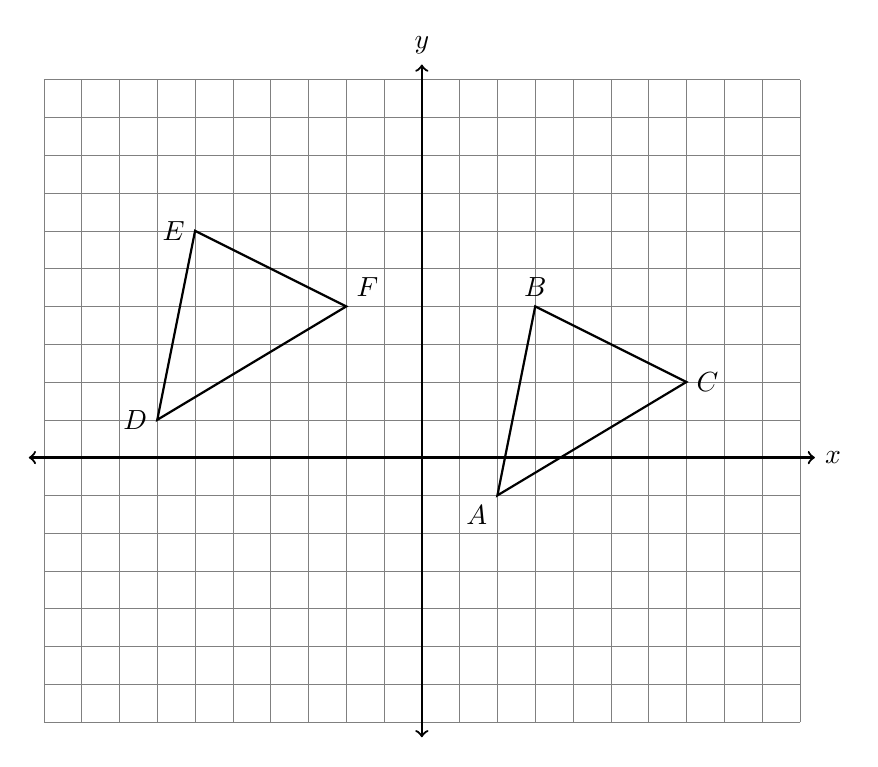
\begin{tikzpicture}[scale=.48]
        \draw [help lines] (-10,-7) grid (10,10);
        \draw [thick, <->] (-10.4,0) -- (10.4,0) node [right] {$x$};
        \draw [thick, <->] (0,-7.4)--(0,10.4) node [above] {$y$};
        \draw [thick]
          (2,-1) node[below left] {$A$}--
          (3,4) node[above] {$B$}--
          (7,2) node[right] {$C$}--cycle;
        \draw [thick]
          (-7,1) node[left] {$D$}--
          (-6,6) node[left] {$E$}--
          (-2,4) node[above right] {$F$}--cycle;
      \end{tikzpicture}
    \end{center}

\newpage
  \item Dilate the $\triangle PQR$ by a factor of $2$ centered at $(4,2)$, drawing its image $\triangle P'Q'R'$ and labeling its vertices.
    \begin{center}
      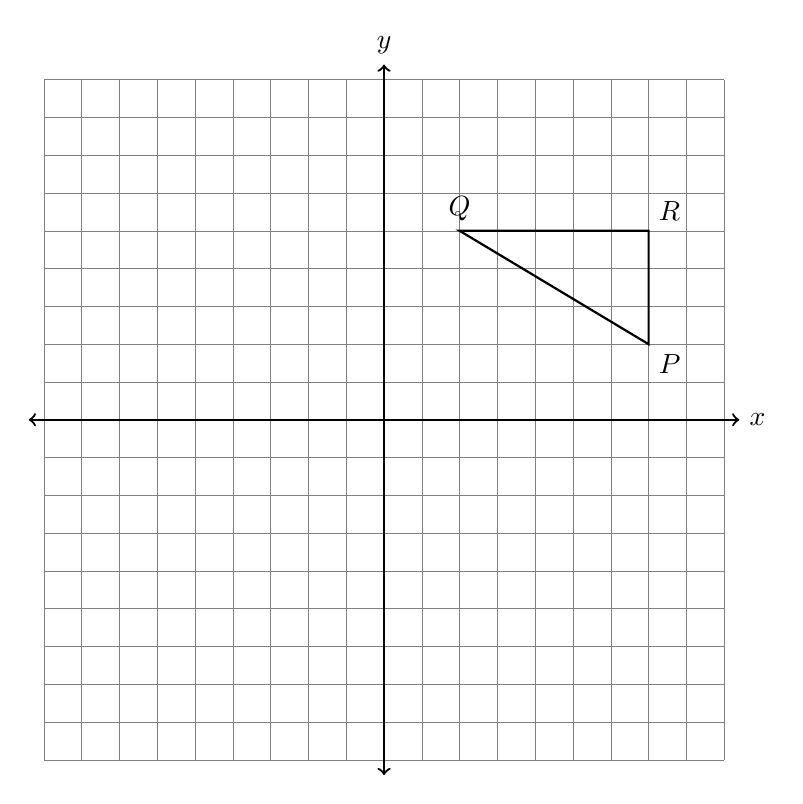
\begin{tikzpicture}[scale=.48]
        \draw [help lines] (-9,-9) grid (9,9);
        \draw [thick, <->] (-9.4,0) -- (9.4,0) node [right] {$x$};
        \draw [thick, <->] (0,-9.4)--(0,9.4) node [above] {$y$};
        \draw [thick]
          (7,2) node[below right] {$P$}--
          (2,5) node[above] {$Q$}--
          (7,5) node[above right] {$R$}--cycle;
      \end{tikzpicture}
    \end{center}

\end{enumerate}
\end{document}
